\documentclass[letterpaper,10pt]{extarticle}
\usepackage[utf8]{inputenc}
\usepackage[T1]{fontenc}
\usepackage{graphicx}
\usepackage[x11names]{xcolor}
\usepackage{tikz}
\usetikzlibrary{circuits.ee.IEC}
\usepackage[os=win]{menukeys}

\usepackage{amsmath,amssymb,textcomp}
\everymath{\displaystyle}

\usepackage{physics}

\usepackage{times}
\renewcommand\familydefault{\sfdefault}
\usepackage{tgheros}
\usepackage{droidmono}

\usepackage{enumitem}
\usepackage[explicit]{titlesec}

\usepackage{multicol}
\setlength{\columnseprule}{0pt}
\setlength{\columnsep}{15.0pt}
\usepackage{multirow}
\usepackage[mode=buildnew]{standalone}
\usepackage{siunitx}

\usepackage{geometry}
\geometry{left=10mm,right=10mm,top=10mm,bottom=15mm,showframe=false}

% custom title
\makeatletter
\renewcommand*{\maketitle}{%
\noindent
\begin{minipage}{0.82\textwidth}

\begin{tikzpicture}
\node[rectangle,rounded corners=6pt,inner sep=6pt,fill=SteelBlue1,text width=.95\textwidth] {\color{black}\huge \@title};
\end{tikzpicture}
\end{minipage}
\hfill
\begin{minipage}{0.17\textwidth}
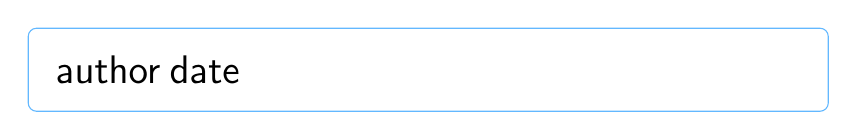
\begin{tikzpicture}
\node[rectangle,rounded corners=3pt,inner sep=10pt,draw=SteelBlue1,text width= 0.78\textwidth] {\raggedleft \Large \@author\ \@date};
\end{tikzpicture}
\end{minipage}
%\bigskip%\bigskip
}%
\makeatother

% custom section
\newcommand*\sectionlabel{}
\titleformat{\section}
  {\gdef\sectionlabel{}
   \normalfont\sffamily\Large\bfseries\scshape}
  {\gdef\sectionlabel{\thesection\ }}{0pt}
  {
\noindent
\begin{tikzpicture}
\node[rectangle,rounded corners=3pt,inner sep=4pt,fill=DodgerBlue4,text width= 0.95\columnwidth] {\color{white}\sectionlabel#1};
\end{tikzpicture}
  }
\titlespacing*{\section}{0pt}{1pt}{0.5pt}

% custom subsection
\newcommand*\subsectionlabel{}
\titleformat{\subsection}{\normalfont\sffamily\bfseries\scshape}{\subsectionlabel}{0pt}{
\noindent
\begin{tikzpicture}
\node[rectangle,rounded corners=4pt,inner sep=3pt,fill=DodgerBlue3,text width= 0.95\columnwidth] {\color{white}\subsectionlabel#1};
\end{tikzpicture}
}
\titlespacing*{\subsection}{0pt}{.5pt}{.5pt}

% custom subsubsection
\newcommand*\subsubsectionlabel{}
\titleformat{\subsubsection}{\normalfont\sffamily\small\bfseries\scshape}{\subsubsectionlabel}{0pt}{
\noindent
\begin{tikzpicture}
\node[rectangle,rounded corners=3pt,inner sep=3pt,fill=blue!50!yellow,text width= 0.95\columnwidth] {\color{white}\subsubsectionlabel#1};
\end{tikzpicture}
}
\titlespacing*{\subsubsection}{0pt}{.5pt}{.5pt}


\title{PHY335 : Physique des ondes}
\author{Final}
\date{E2019}

%\linespread{1.3}

\begin{document}
\maketitle

\begin{multicols*}{2}

\setlength{\belowdisplayskip}{2.5pt}
\setlength{\belowdisplayshortskip}{2.5pt}
\setlength{\abovedisplayskip}{2.5pt}
\setlength{\abovedisplayshortskip}{2.5pt}

\section{Variables}
\vspace{-2em}
\begin{tabular}{lll}
    % Valeur & Formule & Unitée\\\hline
    Amplitude (module) & $A$ & m\\
    Fréquence & $f = 1/T$ & Hz\\
    Fréq. angulaire & $\omega = 2\pi f = 2\pi/T$ & rad/s\\
    Période & $T=1/f$ & s\\
    Déphasage & $\phi$ & rad\\
    \hfill Rappel: & $\cos(\phi)=\sin(\phi + \pi/2)$ & 
\end{tabular}
% \input{sys_masse_ressort.tex}
\section{Mouvement harmonique simple}
\vspace{-2\baselineskip}
\begin{center}
    \includestandalone[scale=1.25]{fig/mhs_graph}
\end{center}

% \subsection{Superposition de MHS}
% \subsubsection{Même fréquence et même direction}
% \centering
% \begin{tabular}{l|l}
%     Objectif &  \(x_R(t)=\sum x_i(t)\)\\\hline
%      & \(a_R=\sum A_i\cos(\phi_i)\)\\
%      & \(b_R=\sum A_i\sin(\phi_i)\)\\
%      & \(A_R=\sqrt{a_R^2+b_R^2}\)\\
%      & \(\phi_R=\tan^{-1}\frac{b_R}{a_R}\)\\[8pt]\hline
%     Résultat & \(x_R(t)=A_R\cos(\omega t + \phi_R)\) 
% \end{tabular}

% \raggedright
% \subsubsection{Même fréquence et directions perpendiculaires}
% Solution:
% \begin{equation*}
%     \qty(\frac{x}{A_x})^2+\qty(\frac{y}{A_y})^2-\frac{2xy}{A_x A_y}\cos(\phi_y-\phi_x)=\sin^2(\phi_y-\phi_x)
% \end{equation*}
% Inclinaison:
% \begin{equation*}
%     \tan(2\alpha)=\frac{2A_x A_y}{A_x^2-A_y^2}\cos(\phi_y-\phi_x)
% \end{equation*}

% \subsubsection{Même fréquence et direction quelconques}
% \begin{center}
%     \includestandalone[scale=1]{fig/mhs_rand_dir}
% \end{center}
% \begin{enumerate}[nosep]
%     \item Décomposer le MHS selon X et Y.
%     \item Additionner les composantes de MHS selon X et Y.
%     \item Combiner les résultantes perpendiculaires.
% \end{enumerate}

% \subsubsection{Fréquences différentes et directions perpendiculaires}
% Dépend de: \( \frac{A_x}{A_y}\), \(\frac{\omega_x}{\omega_y}\) et \(\Delta\phi=\phi_y-\phi_x\)\\
% Résolution par analyse de Fourier.
\section{Mouvement Ondulatoire}
\vspace{-2\baselineskip}
\subsection{Onde sinusoïdale}

\begin{tabular}{lll}
Valeur & Formule & Unitée \\\hline
Longueur d'onde & \(\lambda = cT = c/f\) & m \\%[5pt]
Vitesse de propagation & \(c=\sqrt{F/\mu} \) & m/s \\%\hline\rule{0pt}{15pt}\hspace{-6pt} 
Const. de propagation & \(k = \omega/c = 2\pi/\lambda\)& m$^{-1}$\\
Densité lin. & \(\mu = F/c^2\) & kg/m\\
Vitesse max. & \( v_{\textit{max}}=\omega A\) & m/s\\%[5pt]\hline\rule{0pt}{15pt}
\end{tabular}%
% }


\subsection{Équations du mouvement}
\begin{align*}
    y(x,t) &= A\sin (\omega t \pm kx+\phi)\\
    v(x,t) &=\omega A\cos (\omega t \pm kx+\phi)\\
    a(x,t) &= -\omega^2 A\sin (\omega t \pm kx+\phi)
\end{align*}
\subsubsection{Sens de propagation}
\begin{center}
    \begin{tabular}{cl}
        $-$ & vers la droite ($x>0$)\\
        $+$ & vers la gauche ($x<0$)
    \end{tabular}
\end{center}

% \subsection{Impédance}
% \begin{gather*}
%     Z=\frac{Fk}{\omega} =\frac{F}{c} =\mu c =\sqrt{\mu F}
% \end{gather*}

% \subsection{Puissance}
% \begin{align*}
%     W_{\textit{inst}} &= Z(\omega A)^2\cos^2(\omega t \pm kx +\phi)\\
%     W_{\textit{moy}} &= \frac{Z(\omega A)^2}{2}
% \end{align*}


% \subsection{Interférence dans le plan}
% \begin{center}
%     \includestandalone[scale=1.25]{fig/interference}
% \end{center}
% \[y(P,t)=A_R \cos (\omega t +\phi_R)\]
% \[A_R^2=A_1^2+A_2^2+2A_1 A_2\cos (\psi_2-\psi_1) \]
% \[(\psi_2-\psi_1)=-k(x_2-x_1)+(\phi_2-\phi1)\]

% % \subsubsection{Interférence constructive \hfill$\cos(\psi_2 - \psi_1)>0$}
% % \begin{equation*}
% %     (x_2-x_1)=m\lambda + \frac{\phi_2-\phi_1}{k}
% % \end{equation*}

% % \subsubsection{Interférence destructive \hfill $\cos(\psi_2 - \psi_1)<0$}
% % \begin{equation*}
% %     (x_2-x_1)=(2m+1)\frac{\lambda}{2}+\frac{\phi_2-\phi_1}{k}
% % \end{equation*}


% \begin{tabular}{lll}
%     Type & $\cos(\psi_2 - \psi_1)$ & Équation\\\hline
%     Cons. & $>0$ & \((x_2-x_1)=m\lambda + \frac{\phi_2-\phi_1}{k}\)\\
%     Dest. & $<0$ & \((x_2-x_1)=(2m+1)\frac{\lambda}{2}+\frac{\phi_2-\phi_1}{k}\)
% \end{tabular}



% \subsection{Réflexion et transmission}
% % \subsubsection{Équations}
% \begin{center}
%     \includestandalone[scale=1]{fig/reflex_trans}
% \end{center}
% \begin{tabular}{ll|l}
%     & Milieu 1 & Milieu 2\\\hline
%     incidente & \(y_i=A_i\sin (\omega t - k_1 x)\) &  \multirow{2}{*}{\(y_t=A_t \sin (\omega t-k_2 x) \)} \\
%     réfléchie &\(y_r=A_r\sin (\omega t + k_1 x)\) & \\\hline
%     & \(y_1=y_i+y_r\) & \(y_2=y_t\)
% \end{tabular}

% \subsubsection{Coefficients}
% \begin{tabular}{c|c}
%     Amplitude & Puissance\\\hline
%     \(r=\frac{Z_1-Z_2}{Z_1+Z_2}\) &  \(R=\frac{W_r}{W_i}=\qty(\frac{A_r}{A_i})^2=r^2=\qty(\frac{Z_1-Z_2}{Z_1+Z_2})^2\)\\\rule{-2.5pt}{20pt}
%     \(t=\frac{2Z_1}{Z_1+Z_2}\) & \(T=\frac{W_t}{W_i}=\qty(\frac{A_t}{A_i})^2=\frac{Z_2}{Z_1}t^2=\frac{4Z_1 Z_2}{(Z_1+Z_2)^2}\)
% \end{tabular}
% \begin{tabular}{lll}
%     Caractérisation & Indicateur & Cas extrème\\\hline
%     Réflexion dure & \(Z_2>Z_1\) & \(Z_2=0\)\\
%     Réflexion molle & \(Z_2<Z_1\) & \(Z_2=\alpha\)
% \end{tabular}

% \subsection{Ondes stationnaires}
% % \subsubsection{Équations}
% \begin{align*}
%     y_r &= A\sin (\omega t +kx)\\ 
%     y_i &= -A\sin (\omega t - kx)\\
%     y(x,t)&=2A\sin (kx) \cos (\omega t)
% \end{align*}

% \subsubsection{Noeuds et Ventres}
% \begin{tabular}{l|ll}
%     Noeuds & \(x=\frac{n\lambda}{2}\) & \multirow{2}{*}{\(\mid n = 0,1,2,3,\ldots\)}\\
%     Ventres &  \(x=(2n+1)\frac{\lambda}{4}\) &
% \end{tabular}
% \subsubsection{Combinaison d'ondes stationnaires}
% \begin{tabular}{ll}
%     Fondamantale & \(\lambda_n = \frac{2L}{n}\) \\\rule{-2.5pt}{15pt}
%     Harmoniques & \(f_n=\frac{nc}{2L}\)
% \end{tabular}
\section{Nature et propag. lumière}
\vspace{-2\baselineskip}
\subsection{Constantes physique}
\begin{tabular}{lccc}
Nom                                & Symb.                                                       & Valeur & Unité                                                                                                                                                                                  \\ 
\hline
Perméabilité (vide)               & $\mu_0$                                     & \num{4\pi e-7} & \si{T.m\per A}                                  \\
Permittivité (vide)               & $\varepsilon_0$ & \num{8,854e-12} & \si {\coulomb\squared\per(N.m^2)}  \\
V. lumière (vide) & $c_0$                                                         & \num{3,00e8} & \si{\meter\per\second}                                                                           
\end{tabular}

\begin{tabular}{lll}
Valeur & Formule & Unitée \\\hline
C. élec. & \(E_x(z,t)=E_o\sin (\omega t \pm k z + \phi_o)\) & \si{\volt\per\meter} \\[3pt]
C. magn. & \(B_y(z,t)=B_o\sin (\omega t \pm k z +\phi_o)\) & \si{\tesla}\\[3pt]
Rapport & \(c=\frac{E_o}{B_o}\) &
\end{tabular}

\subsection{Vecteur de Poynting ou intensité de l'OEM}
\begin{tabular}{ll}
\(S=I=\frac{EB}{\mu_o}\) & \si{\watt\per\meter\squared}\\[8pt]
\(I_{\textit{moy}}=\frac{E_o B_o}{2\mu_o} = \frac{E_o^2}{2 \mu_o c_o}=\frac{c_o B_o^2}{2\mu_o}\) & \si{\watt\per\meter\squared}
\end{tabular}


\subsection{Rayonnement d'un corps noir}
\subsubsection{Loi de Wien}
\begin{tabular}{lll}
    % Valeur & Formule & Unitée \\\hline
    Rayonnement émis &  \(\lambda_{\text{max}}=2.898\times 10^{-3}/T\) & \si{\micro\meter}\\
    \hfill Rappel: & \(T_K=T_c+273\) & \si{\kelvin}
\end{tabular}

\subsubsection{Loi de Stefan-Boltzmann}
\begin{tabular}{lll}
% Valeur & Formule & Unitée\\\hline
    Luminosité & \(L=IA\) & \si{\watt}\\
    Intensité & \(I= 5.67\times10^{-8} (T^4-T_0^4)\) & \si{\watt\per\meter\squared}
\end{tabular}
\subsection{Quantité de mouvement d'un photon}
\begin{center}
\begin{tabular}{ll}
    \(p=\frac{E}{c}\) & \si{\kilo \gram \meter\per\second}
\end{tabular}
\subsubsection{Énergie des photons (pblm type: Photons émis)}
\(E = nhf\) \si{\watt} \(|\ h=6.625\times10^{-34} \) \si{\J\second}\\
\end{center}
\subsection{Quantité de mouvement sur une surface}
\begin{tabular}{lll}
    absorbante &  \(p=U/c\) & \si{\kilo \gram \meter\per\second}\\
    réfléchissante & \(p=2U/c\) & \si{\kilo \gram \meter\per\second}\\
    générale & \(p=(R+1)\frac{U}{c}\) & \si{\kilo \gram \meter\per\second}
\end{tabular}

\subsubsection{Pression de radiation}
\begin{tabular}{lll}
    Pression & \(P=\frac{(R+1)}{c}I_{\text{moy}}\) & \si{\newton\per\meter\squared}\\[5pt]
    \hfill Rappel: & \(P=F/A\) et \(F=ma\) &
\end{tabular}


\subsection{Effet Doppler}
\includestandalone[width=.45\textwidth]{fig/doppler}
\[\vec{v}=\vec{v_s}-\vec{v_o}\]
\begin{tabular}{ll}
    \(v>0\) &  \(f_o=f_s\qty(\frac{\sqrt{1-\qty(\frac{v}{c})^2}}{1+\frac{v}{c}\cos (\theta)})\)
\end{tabular}
% \[f_o=f_s\qty(\frac{\sqrt{1-\qty(\frac{v}{c})^2}}{1+\frac{v}{c}\cos (\theta)})\]
%\[f_o=f_s\sqrt{1-\qty(\frac{v}{c})^2} \qquad f_o<f_s\]

\subsubsection{Déplacement Doppler}
\[\vec{\Delta\lambda}=\vec{\lambda_o}-\vec{\lambda_s}\]
\[\lambda_o=\lambda_s\qty(\frac{1+\frac{v}{c}\cos (\theta)}{\sqrt{1-\qty(\frac{v}{c})^2}})\]
\[\frac{ \Delta\lambda }{\lambda_s}=\frac{1+\frac{v}{c}\cos (\theta)}{\sqrt{1-\qty(\frac{v}{c})^2}}-1\]
Pour \(\frac{v}{c} <<< 1\): \(\frac{\Delta \lambda}{\lambda_s}=\frac{v}{c}\cos (\theta)\)
% \section{Optique physique}
\vspace{-2\baselineskip}
\subsection{Convention de signe}
\begin{tabular}{cl}
    $S_o > 0$ & objet réel \\
    $S_o < 0$ & objet virtuel\\\hline
    $S_i > 0$ & image réelle\\
    $S_i < 0$ & image virtuelle\\\hline
    $R > 0$ & centre de courbure $C$ du côté émergent\\
    $R < 0$ & $C$ du côté incident\\\hline
    $g_t > 0$ & image droite\\
    $g_t < 0$ & image renversée\\\hline
    $f>0$ & lentille convergente\\
    $f<0$ & lentille divergente
\end{tabular}
% \section{Optique géo. surfaces planes}
\vspace{-2\baselineskip}
\begin{tabular}{ll}
    Valeur & Formule \\\hline
    Indice de réfraction & \(n=c_o/c\)\\
    Rayon réfracté & \(n_i\sin{\theta_i} = n_t\sin{\theta_t}\)\\[2pt]
    Profondeur apparante & \(\frac{y^\prime}{y}=\frac{n_t}{n_i}\)\\[8pt]
    Réflextion totale interne & \(\sin{\theta_c}=\frac{n_t}{n_i}\)\\
    Angle critique & $\theta_c$
\end{tabular}

\begin{gather*}
    n_{\textsc{air}}=1.0 \qquad n_{\textsc{eau}}=1.33 \qquad n_{\textsc{verre}}=1.5
\end{gather*}

\subsection{Plaques parallèles}
\begin{align*}
    n_1\sin{\theta_i} &= n_f\sin{\theta_t}\\
    n_1 &= n_f\\
    \theta_i &= \theta_t
\end{align*}
% \section{Optique géo. surfaces courbes}
\vspace{-2\baselineskip}
\subsection{Dioptre}
\begin{tabular}{ll}
    Lentille &  \(\frac{n_i}{s_o}+\frac{n_t}{s_i}=\frac{n_t-n_i}{R}\)\\[8pt]
    Miroir & \(\frac{1}{s_o}+\frac{1}{s_i}=\frac{2}{R}=\frac{1}{f}\)
\end{tabular}

% \[\frac{n_i}{s_o}+\frac{n_t}{s_i}=\frac{n_t-n_i}{R}\]
% \subsubsection{Cas particulier: Miroir}
% \[\frac{1}{s_o}+\frac{1}{s_i}=\frac{2}{R}\]

% \subsubsection{Distance focale}
% \[\frac{1}{s_o}+\frac{1}{s_i}=\frac{2}{R}=\frac{1}{f}\]
\subsection{Foyers}
\begin{tabular}{ll}
    Objet & \(f_o = \frac{n_i R}{n_t-n_i} \) \\
    Image & \(f_i = \frac{n_t R}{n_t-n_i} \)
\end{tabular}

\subsection{Lentille mince}
\begin{align*}
    \frac{1}{s_i}+\frac{1}{s_o}&=\frac{n_l-n_a}{n_a}\qty(\frac{1}{R_1}+\frac{1}{R_2})\\
    \frac{1}{s_i}+\frac{1}{s_o}&=(n_{la}-1)\qty(\frac{1}{R_1}+\frac{1}{R_2})
\end{align*}

\subsection{Lentille épaisse}
\includegraphics[width=.45\textwidth]{fig/thk_lens.PNG}
\[\frac{1}{s_i}+\frac{1}{s_o}=\frac{1}{f} = (n_{la}-1)\qty(\frac{1}{R_1}-\frac{1}{R_2}+\frac{(n_{la}-1)a}{n_{la}R_1R_2})\]
% $a$ est l'épaisseur de la lentille.
\subsubsection{Plans principaux}
$V$ vers $H$ dans le sens de la propagation.
\begin{align*}
    \overline{V_1H_1} &= \frac{-f(n_{la}-1)a}{R_2n_{la}}\\
    \overline{V_2H_2} &= \overline{V_1H_1}\frac{R_2}{R_1}
\end{align*}

\subsection{Grandissement}
\begin{tabular}{ll}
    Grandissement &  \(g_t = \frac{-n_i s_i}{n_t s_o} = \frac{h_i}{h_o}=\frac{-s_i}{s_o}\) \\[8pt]
    Grandissement total & \(g_t=g_{t_{1}}\times g_{t_{2}} \times \ldots = \frac{h_i}{h_o}\)
\end{tabular}

\subsection{Combinaison de lentilles}
\centering
\includegraphics[trim={.75cm 0 1cm 0},clip=true, width=.4\textwidth]{fig/lens_comb.tex}
\[s_{o_2}=d_a-s_{i_1}\]

\raggedright
\section{Interférence}
\subsection{Cas général}
\subsubsection{Différence de marche}
\[\delta=\qty[\sum_in_id_i]_2-\qty[\sum_ini_di]_1+(p_2-p_1)\frac{\lambda_o}{2}+\frac{\lambda_o(\phi_2-\phi_1)}{2\pi}\]

\subsubsection{Intensité}
\[I=I_1+I_2+2\sqrt{I_1I_2}\cos{\theta}\cos(\psi_2-\psi_1) \]
\[(\psi_2-\psi_1)=k_o\delta=k_o(r_2-r_1)\]
% \[k_o=\frac{2\pi}{\lambda}\]


\subsection{Fentes de Young}
\begin{center}
    \includestandalone[width=.46\textwidth]{fig/young}
\end{center}
\begin{tabular}{ll}
    Constructive & \(\delta=m\lambda=d\sin{\theta}\)\\
    Destructive & \(\delta=(2m+1)\frac{\lambda}{2}=d\sin{\theta}\)\\[8pt]
    Dist. intensité & \(I=4I_o\cos^2\qty(\frac{k_o\delta}{2}) \)\\[8pt]
    Visibilité (Contraste) & \(V=\frac{2\sqrt{I_1I_2}}{I_1+I_2}\)
\end{tabular}



\subsection{Lames à faces parallèles (air-verre-air)}
\begin{center}
    \includegraphics[height=.2\textwidth]{fig/parallel.PNG}
\end{center}
\begin{tabular}{ll}
    Différence de marche & \(\delta=2ne-\frac{\lambda_o}{2}\)\\
    Constructif & \(2e=(m+1/2)\frac{\lambda_o}{n}\) \\
    Destructif & \(2e=m\frac{\lambda_o}{n}\)
\end{tabular}

\subsection{Lames à faces presque parallèles (air-verre-air)}
\begin{center}
    \includegraphics[width=0.35\textwidth]{fig/lames_presque_paralleles.PNG}    
\end{center}
% \vspace{-1\baselineskip}
\begin{tabular}{ll}
    Différence de marche & \(\delta=2ne-\frac{\lambda_o}{2}=2n\alpha x - \frac{\lambda_o}{2}\)\\[8pt]
    Constructif & \(x_c=(m+1/2)\frac{\lambda_o}{2\alpha n}\)\\[8pt]
    Destructif & \(x_d=\frac{m\lambda_o}{2\alpha n}\)\\[8pt]
    Dist. entrée-sortie & \(\Delta x = \frac{\lambda_o}{2\alpha n}\)
\end{tabular}


\subsection{Interféromètre de Michelson}
\begin{center}
    \includegraphics[width=.35\textwidth]{fig/michelson.png}
\end{center}
\begin{tabular}{ll}
    Différence de marche & \(\delta=2(d_2-d_1)\)\\
    Constructif & \(2(d_2-d_1)=m\lambda_o\) \\
    Destructif & \(2(d_2-d_1)=(2m+1)\frac{\lambda_o}{2}\)
\end{tabular}
\section{Nature et propagation du son}
\subsection{Vitesse du son dans divers milieux}
% \begin{tabular}{lll}
% Vitesse de propagation & \(c=\sqrt{B/\rho} \) & m/s \\%\hline\rule{0pt}{15pt}\hspace{-6pt} 
% \end{tabular}
\begin{tabular}{ll|ll}
    Milieux & c (\si{\meter\per\second}) & Milieux & c (\si{\meter\per\second})\\\hline
    Air (\SI{0}{\degreeCelsius}) & 331 & Eau de mer & 1533\\
    Air (\SI{100}{\degreeCelsius} & 366 & Aluminium & 5100\\
    Hydrogène (\SI{0}{\degreeCelsius}) & 1286 & Cuivre & 3560\\
    Oxygène (\SI{0}{\degreeCelsius}) & 317 & Fer & 5130\\
    Hélium (\SI{0}{\degreeCelsius}) & 972 & Plomb & 1322\\
    Eau & 1493 & Alcool & 1143
\end{tabular}

\subsection{Fonctions d'ondes}
\begin{tabular}{lll}
% Valeur & Formule & Unité\\\hline
    Déplacement &  \(u(x,t)=A\sin (\omega t \pm kx+\phi)\) & \si{\meter}\\[5pt]
    Pression & \(p(x,t)=P_{o}\cos(\omega t \pm kx+\phi)\) & \si{\pascal}\\[5pt]
    Amplitude & \(P_{o}=\rho c \omega A\) & \si{\pascal}\\[5pt]
    Impédance & \(Z=P/V=\sqrt{B\rho}=\rho c\) & \si{\pascal\second\per\meter}\\[5pt]
    V. propagation & \(c=\sqrt{B/\rho} \) & \si{\meter\per\second}
\end{tabular}

\subsection{Intensité d'une onde}
\begin{center}
\begin{tabular}{c|c}
    Onde plane & Onde sphérique \\\hline\\[-1em]
    \(I=\frac{\rho c (\omega A)^2}{2}=\frac{P_{o}^{2}}{2\rho c}\) & \(I=\frac{W}{S}=\frac{W}{4\pi r^{2}}\)
\end{tabular}
\hspace{1em}\si{\watt\per\meter\squared}
\end{center}

% \subsubsection{Onde plane}
% \begin{center}
%     \(I=\frac{\rho c (\omega A)^2}{2}=\frac{P_{o}^{2}}{2\rho c}\) \si{\watt\per\meter\squared}    
% \end{center}

% \subsubsection{Onde sphérique}
% \begin{center}
%     \(I=\frac{W}{S}=\frac{W}{4\pi r^{2}}\) \si{\watt\per\meter\squared}    
% \end{center}

\subsection{Intensité en décibel}
\begin{center}
    \(IL=10\log\qty(\frac{I}{10^{-12}})=10\log(I)+120\) \si{\decibel}    
\end{center}

\subsection{Onde stationnaire}
% \begin{tabular}{lll}
% %Valeur & Formule & Unité\\\hline
% Déplacement & \(u(x,t)=2A\sin(kx)\cos(\omega t)\) & \si{\meter}\\
% Pression & \(P(x,t)=2P_{o}\cos(kx)\sin(\omega t)\) & \si{\pascal}
% \end{tabular}

\subsubsection{Colonne fermée aux deux extrémités (Cas général)}
\begin{tabular}{lll}
Longueur de colonne & \(L=\frac{n\lambda}{2}\) & \si{\meter}\\[8pt]
Longueur d'onde & \(\lambda_{n}=\frac{2L}{n}\) & \si{\meter}\\[8pt]
Fréquence & \(f_{n}=\frac{nc}{2L}\) & \si{\hertz}\\[8pt]
Déplacement & \(u(x,t)=2A\sin(kx)\cos(\omega t)\) & \si{\meter}\\[5pt]
Pression & \(P(x,t)=2P_{o}\cos(kx)\sin(\omega t)\) & \si{\pascal}
\end{tabular}

\subsubsection{Colonne ouverte aux deux extrémités}

\begin{tabular}{lll}
% Valeur & Formule & Unité\\\hline
% Longueur de colonne & \(L=\frac{n\lambda}{2}\) & \si{\meter}\\[8pt]
% Longueur d'onde & \(\lambda_{n}=\frac{2L}{n}\) & \si{\meter}\\[8pt]
% Fréquence & \(f_{n}=\frac{nc}{2L}\) & \si{\hertz}\\[8pt]
Déplacement & \(u(x,t)=2A\cos(kx)\sin(\omega t)\) & \si{\meter}\\[5pt]
Pression & \(P(x,t)=2P_{o}\sin(kx)\cos(\omega t)\) & \si{\pascal}
\end{tabular}

% \subsubsection{Colonne fermée aux deux extrémités}
% \begin{tabular}{lll}
% Longueur de colonne & \(L=\frac{n\lambda}{2}\) & \si{\meter}\\[8pt]
% Longueur d'onde & \(\lambda_{n}=\frac{2L}{n}\) & \si{\meter}\\[8pt]
% Fréquence & \(f_{n}=\frac{nc}{2L}\) & \si{\hertz}\\[8pt]
% Déplacement & \(u(x,t)=2A\sin(kx)\cos(\omega t)\) & \si{\meter}\\[5pt]
% Pression & \(P(x,t)=2P_{o}\cos(kx)\sin(\omega t)\) & \si{\pascal}
% \end{tabular}

\subsubsection{Colonne ouverte à une extrémité, fermée à l'autre}
\begin{tabular}{lll}
Longueur de colonne & \(L=(2n-1)\frac{\lambda}{4}\) & \si{\meter}\\
Longueur d'onde & \(\lambda_{n}=\frac{4L}{(2n-1)}\) & \si{\meter}\\[8pt]
Fréquence & \(f_{n}=\frac{(2n-1)c}{4L}\) & \si{\hertz}\\[8pt]
Déplacement & \(u(x,t)=2A\cos(kx)\sin(\omega t)\) & \si{\meter}\\[5pt]
Pression & \(P(x,t)=2P_{o}\sin(kx)\cos(\omega t)\) & \si{\pascal}
\end{tabular}

\subsection{Battement}
\begin{align*}
    P&=P_{o_{1}}\cos(\omega_1 t)+P_{{o}_{2}}\cos(\omega_2 t)\\
    P(t)&=2P_{o}\cos\qty(\frac{\omega_1-\omega_2}{2}\,t)\cos\qty(\frac{\omega_1+\omega_2}{2}\,t)
\end{align*}
\[\bar{f}=\frac{1}{2\pi}\qty(\frac{\omega_1+\omega_2}{2})=\frac{f_1+f_2}{2}\]


\subsection{Effet Doppler}
\begin{center}
    \includegraphics[width=0.25\textwidth]{fig/doppler.PNG}    
\end{center}
% \vspace{-1\baselineskip}
\[f_{o}=f_{s}\qty(\frac{c+v_{v}\cos(\gamma)-v_{o}\cos(\alpha)}{c+v_{v}\cos(\gamma)-v_{s}\cos(\beta)})\]
\begin{tabular}{ll|ll}
    Fréq. observée & \(f_{o}\) & Vitesse vent & \(v_{v}\)  \\
    Fréq. source & \(f_{s}\) & Vitesse source & \(v_{s}\) \\
    & & Vitesse observateur & \(v_{o}\)
\end{tabular}
% \section*{Cercle trigonométrique}
% \begin{center}
%     \includegraphics[width=0.3\textwidth]{fig/unit_circle.png}    
% \end{center}

\section*{Préfixes Système International}
\begin{center}
% \begin{tabular}{lll}
% Facteur    & Nom   & Symbol \\\hline\\[-1em]
% $10^{6}$   & mega  & M      \\
% $10^3$     & kilo  & k      \\
% $10^{-3}$  & milli & m      \\
% $10^{-6}$  & micro & $\mu$  \\
% $10^{-9}$  & nano  & n      \\
% $10^{-12}$ & pico  & p     
% \end{tabular}

\begin{tabular}{lll|lll}
Facteur    & Nom   & Symbol & Facteur    & Nom   & Symbol \\\hline\\[-1em]
$10^{6}$   & mega  & M & $10^{-6}$  & micro & $\mu$ \\
$10^3$     & kilo  & k & $10^{-9}$  & nano  & n     \\
$10^{-3}$  & milli & m & $10^{-12}$ & pico  & p
\end{tabular}

\end{center}

% \section*{Cercle trigonométrique}
\begin{center}
    \includegraphics[width=0.35\textwidth]{fig/unit_circle.png}    
\end{center}


\end{multicols*}

\end{document}
